% !TeX spellcheck = da_DK
\section{Systembeskrivelse}
For at gøre anvendelse af samme system muligt til 4. Semester skal arbejdsområdet kunne benyttes sammen med et USB-baseret trådløst udviklingsværktøj eZ430-RF2500 fra Texas Instruments. Det er derfor nødvendigt, at designet stemmer overens med udviklingsværktøjet for at kunne sende og modtage data til og fra computeren. Udviklingsværktøjet indeholder hardware og software som evaluerer mikrokontrolleren MSP430F2274. For at hele vores system kan anvendes med udviklingsværktøjet, skal outputsignalet være 3V, eftersom mikrokontrolleren opererer med spændingsforsyning mellem 1,8V og 3,6V.  

\subsection{Formål og anvendelse}
Ud fra problemanalysen fremgår det, at ældre over 65 år i højere grad får apopleksi, hvortil balanceproblemer er en hyppig gene. Derudover har apopleksipatienter ofte kognitive problemer. Apopleksipatienter har et ønske om at være selvstændige og uafhængige. 

Systemet skal opfange, hvis patienten er ude af balance og være nemt anvendeligt, da det skal bruges til selvtræning af balancen i hjemmet - altså implementeres i fase 4, som bliver omtalt på side \pageref{Faser}. For at systemet kan anvendes af målgruppen, skal det være brugervenligt - dvs. let at påsætte, ikke veje for meget samt signalerne skal være let forståelige. Målgruppen giver yderligere begrænsninger ift. feedback, da både hørelsen, synet eller kroppens følelser kan være svækket. Derudover skal systemet kunne give et digitalt output, som er muligt at behandle.


\subsection{Beskrivelse af test}
Patienten skal være stående på en tegnet linje med den ene fods tæer mod den anden fods hæl\fxnote{måske et billede vi tager som vil illustrere dette}. Netop denne position anvendes for at udfordre patientens balance ved at fordele kropsvægten anderledes ift. den normale kropsstilling som bliver omtalt på side \pageref{BalanceAfsnit}. Patienten påsætter systemet og udfører herefter en prøvetest for at kende til den givne feedback. Prøvetesten indebærer, at patienten svajer langsomt fra side til side. Hvis patienten hælder xx, vil en lampe lyse gult og patienten vil kunne mærke vibration. Hvis patienten ikke retter sig op og ender i en riskozone vil en anden lampe lyse rødt. Vibrationen vil stige i takt med at lyset ændrer sig fra gult til rødt. Selve øvelsen udføres herefter ved at holde balancen i udgangspositionen, hvorefter øjenene lukkes. Dette gøres for at udelukke den visuelle sans, hvilket gør det svære for patienten at opretholde balancen. Selve forsøget gentages efter behov. \\
Ved at tage målinger over tid i rehabiliteringsforløbet vil det forventes at der sker en fremgang mellem målingerne. 

\subsection{Optagelse af signal fra accelerometer}
Acceleorometeret skal give et elektrisk signal ud fra den position som anvendes i forsøget \fxnote{Vi skal vurdere hvor signalet kommer fra om det x,y,z aksen.}. Accelerometeret opfanger de signaler som udsendes fra sensoren som er placeret anteriort på patientens brystkasse. Signalet afhænger af, hvor langt patienten har flyttet sig. 

............ HER MANGLER NOGET INFORMATION..........................

Ledningerne snoes for at kontrollere samt mindske støjen. Derudover sættes ledninger fast med tape på patienten, så vidt det er muligt. For at undgå unødvendigt støj foretages forsøget væk fra andet elektronik.  %\ref{reference til støj afsnittet}



\subsection{Analogt output}
Det analoge output skal kunne henvende sig til patienten, dette sker ved lysdioder og vibration. Lysdioderne skal lyse gult ved 'usikkerhed' og slukke hvis patienten enten er rettet op igen eller bevæger sig ud i riskozonen, hvorefter en ny diode skal lyse rødt. Vibrationerne igangsættes ved 'usikkerhed' og skal stoppe hvis patienten retter sig op eller stige i styrke, hvis patienten kommer ud i risikozonen. 

\subsection{Digitalt output}
Det digitale skal kunne anvendes af sundhedspersonale til at vurdere om patienten gør fremskridt, dette indebærer at informationerne for patienten kan gemmes og sammenlignes på en computer. 


\subsection{Systemets opbygning}
Systemets opbygning fremgår af \figref{kravblok}.

\begin{figure}[H]
	\centering
	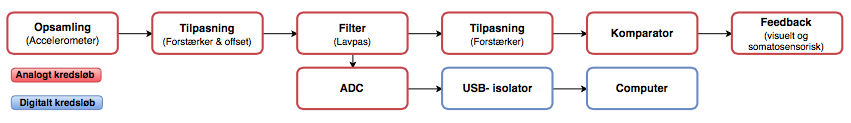
\includegraphics[scale=0.62]{figures/cProblemloesning/blokdiagram1.png}
	\caption{Figuren viser de blokke/elementer som systemet skal indeholde}
	\label{kravblok}
\end{figure}

Signalerne fra accelerometeret skal forstrækes, herefter støj skal filteres fra for at dæmpe uønskede frekvenser. Herefter forstærkes signalet med en variabel forstærkningen, da signalet kun er forstærket lidt. Signalet forstærkes til maksimalt 3V. Dette gøres ved en operationsforstærker \fxnote{inverteret eller ikke-inverteret} Det analoge signal ensrettet via. \fxnote{helbølgeensretter eller halvbølgeensretter}, hvor efter der benyttes en integrator til at lave en lineær linje. Ud fra denne linje gives en advarsel via feedback. Det digitale signal skal konverteres fra analogt til digitalt, hvilket gøres ved en ADC.  Herefter anvendes en USB-isolator for patientsikkerhed. Computeren skal fremvise en graf når NIDAQ er tilsluttet. 

\subsection{Kravspecifikationer}
Til vurdering af tolerance er der udført et pilotforsøg, dette er udført med henblik på at kunne beregne forstærkning, filtrering og integrering af signalet. 

\subsubsection{Det samlede system}
Det analoge output sammenligninger inputtet som kommer fra accelerometeret og outputtet i form af 2 dioder og stigning i vibration. Aktivering af bestemte dioder skal afspejle inputsignalet således at et lille input aktiverer en gul diode og vibration, mens et større input aktiverer en rød diode og stigningen i vibration. 

\textbf{Krav:}
\begin{itemize}
\item Den gule diode skal lyse når patienten har bevæget sig XX og slukke hvis patienten retter sig op eller hælder yderligere.
\item Den røde diode skal lyse når patienten har bevæget sig XX og slukke, hvis patienten retter sig op.
\item Vibration skal igangsættes når patienten har bevæget sig XX og skal slukke, hvis patienten retter sig op eller stige, hvis patienten hælder yderligere.
\item Der skal være en sammenhæng mellem inputsignalets størrelse og antallet af dioder der lyser?
\item Signalet i systemet må ikke forstærkes til en værdi over 3V.
\end{itemize}

%\textbf{Tolerance:}
%\begin{itemize}
%\end{itemize}
%
%\subsubsection{Accelerometer}
%\textbf{Krav:}
%\begin{itemize}
%\end{itemize}
%
%\textbf{Tolerance:}
%\begin{itemize}
%end{itemize}
%
%\subsubsection{Instrumentering forstærker}
%\textbf{Krav:}
%\begin{itemize}
%\end{itemize}
%
%\textbf{Tolerance:}
%\begin{itemize}
%\end{itemize}
%
%\subsubsection{Filtre - opdeling i høj og lavpass?}
%\textbf{Krav:}
%\begin{itemize}
%\end{itemize}
%
%\textbf{Tolerance:}
%\begin{itemize}
%\end{itemize}

%\subsubsection{Forstærker med variabel forstærkning}

%\textbf{Krav:}
%\begin{itemize}
%\end{itemize}
%
%\textbf{Tolerance:}
%\begin{itemize}
%\end{itemize}
%
%\subsubsection{Ensretter}

%\textbf{Krav:}
%\begin{itemize}
%\end{itemize}
%
%\textbf{Tolerance:}
%begin{itemize}
%end{itemize}
%
%\subsubsection{Integrator}
%\textbf{Krav:}
%\begin{itemize}
%\end{itemize}
%
%\textbf{Tolerance:}
%\begin{itemize}
%\end{itemize}
%
%\subsubsection{Advarsel}
%\textbf{Krav:}
%\begin{itemize}
%\end{itemize}
%
%\textbf{Tolerance:}
%\begin{itemize}
%\end{itemize}
%
%\subsubsection{ADC}
%\textbf{Krav:}
%\begin{itemize}
%\end{itemize}
%
%\textbf{Tolerance:}
%\begin{itemize}
%\end{itemize}
%
%\subsubsection{USB-isolator}
%\textbf{Krav:}
%\begin{itemize}
%\end{itemize}
%
%\textbf{Tolerance:}
%\begin{itemize}
%\end{itemize}
%
%\subsubsection{Computer}
%\textbf{Krav:}
%\begin{itemize}
%\end{itemize}
%
%\textbf{Tolerance:}
%\begin{itemize}
%\end{itemize}
%\begin{itemize}
%\item Systemet skal ved fald få dioder til at lyse samt give feedback i form af stigende vibration. 
%\item Systemet skal være non-invasiv - dvs. systemet ikke må påføre patienten smerte eller varig skade
%\item Systemet skal være brugervenligt
%\item Systemet skal forsynes med spænding fra 9V batteri
%\end{itemize}

%\subsubsection{Accelerometer}
%Accelerometeret skal detektere patientens kropshældning.

%\subsubsection{Filter}
%Når der anvendes et filter, skal det dæmpe uønskede frekvenser. Dvs. frekvenser der lavere eller højere ift. det signal fra accelerometeret, som man vil analysere på. Der skal udføres et pilotforsøg for at finde frem til det korrekte filter og valg af knækfrekvens. 

%\subsubsection{Signalerende lys}
%Når patienten er ude af balance skal en rød diode lyse, som signalering ift. patientens hældning. Der skal vha. et pilotforsøg detekteres, hvornår dioden skal lyse. Skal der evt. være 2 dioder, hvor den ene er et "advarende" signal og nr. to er "fare". 

%\subsubsection{Alarm/vibrationen}
%Alarmen/vibrationen skal anvendes i perioden, hvor patienten er ude af balance og stoppe igen, når der igen er oprettet balance. 
%(eller fungere som en alarm til dioderne - så når en diode lyser, skal alarmen gå)

%\subsubsection{ADC}
%Der anvendes en ADC i systemet, for at konvertere det analoge signal til digitalt. Det næste skridt er konverteringen til PC og det er derfor essentielt at have en ADC, der konverterer analogt signal til binære tal, som digitale systemet anvender. 
%{Her skal vi have valgt en samplingsfrekvens)

%\subsubsection{USB-isolater}
%USB-isolatoren sikre patientens sikkerhed. Her skal input- og outputspænding være ens.  

%\subsubsection{Til PC}
%Fremvisning af graf, så patienten og plejepersonale kan følge %rehabiliteringens udvikling. 
